%% retrank @ NTCIR-19 R2C2 --- v2, calibration-first framing, judge-robustness foregrounded.
%% Target: ACM sigconf, <= 8 pages incl. refs. Requires the ACM `acmart' class.
%% NOTE: numbers marked (official) are from data/eval/official/*; (self) are self-evaluated.
\documentclass[sigconf,nonacm]{acmart}

\usepackage{booktabs}
\usepackage{amsmath}

\newcommand{\HMR}{\textsc{HMR}}
\newcommand{\MNP}{\textsc{MNP}}
\newcommand{\RO}{R_{\mathrm{O}}}
\newcommand{\RU}{R_{\mathrm{U}}}

\begin{document}

\title{retrank at the NTCIR-19 R2C2 Task}
\subtitle{Answering with Confidence as a Calibration Problem, and Why an LLM-Judged Win Still Means Something}

\author{Alessandro Magnani}
%% AFFILIATION PENDING EMPLOYER APPROVAL.
%%   If/when the employer approves, swap the line below for the institutional affiliation.
%%   Default (needs no approval): Independent Researcher (active below).
\affiliation{\institution{Independent Researcher}\country{USA}}
\email{ale.magnani@gmail.com}

\renewcommand{\shortauthors}{Magnani}

\begin{abstract}
We report \textbf{retrank}'s submission to the NTCIR-19 R2C2 Answering-with-Confidence
(AC) subtask, scored by the Harmonic Mean of Rewards (\HMR), which jointly penalises
overconfidence on wrong answers ($\RO$) and underconfidence on right ones ($\RU$),
alongside Accuracy and Mean Nugget Precision (\MNP). \textbf{Under official scoring our
four runs took the top four \HMR{} positions among 25 runs from 7 teams (best 0.974,
main system 0.963, vs.\ 0.761 for the strongest other run); retrank's \emph{weakest} run
(0.868) beats every other team's \emph{best}. retrank also ranks first on Accuracy (0.969)
and \MNP{} (0.840, sweeping the top four), the \MNP{} lead significant ($\alpha{=}0.05$)
over every team but BITEM (randomised Tukey HSD~\cite{sakai-sigtest}, $B{=}5000$).} Our thesis is that AC is a \emph{calibration}
problem disguised as a QA problem: a comparably accurate competitor (BITEM) matched our
accuracy (0.92) at half our \HMR{} (0.49), so the gap is primarily confidence discipline
rather than answer quality. We locate the win in \emph{high accuracy paired with confidence
calibrated to it} (best run: mean confidence $0.956$ vs.\ accuracy $0.953$; calibration
error $+0.003$), delivered by an
answer-first pipeline whose confidence is set by an independent verifier rather than the
generator. Because all R2C2 ground truth is LLM-generated (relevance judged by Qwen-3.5
and GPT-5.5) and we tuned against Claude, we confront the natural objection --- ``you won
because you used a strong LLM'' --- directly: (i) our Claude self-evaluator matches the
\emph{official} (Qwen/GPT) \HMR{} of our two main runs to within $0.0004$ \emph{in-sample},
and predicts five \emph{held-out} competitor runs' official \HMR{} with only weak
cross-family correlation ($\rho{=}0.60$ on $n{=}5$, not significant); (ii) our pipeline
run on the \emph{cheapest} Claude tier (all-Haiku) would stay in the competitive range of
the field-leading team \emph{under self-evaluation} --- so the margin is not obviously bought
by model tier.
We argue the lever is a
largely model-agnostic calibration wrapper --- it transfers across competitors' systems and,
when the pipeline is swapped end-to-end (streamlined) onto three GPT models, reproduces the
calibration gain (3/3 positive, one significant) --- with the residual caveat that these checks use a
surrogate rather than the official judge.
\end{abstract}

\keywords{answering with confidence, calibration, HMR, RAG, LLM evaluation}

\maketitle

%% Required NTCIR participant-paper fields.
\noindent\textbf{Team Name:} retrank \quad\textbf{Subtasks:} PR, AC

\section{Introduction}
The NTCIR-19 R2C2 Answering-with-Confidence (AC) subtask asks a system, for each
question, to return an answer, a confidence score in $[0,100]$, and grounded nuggets that
cite passages from any team's passage-retrieval run. Systems are ranked by three official
metrics --- Accuracy, Mean Nugget Precision (\MNP), and the Harmonic Mean of Rewards
(\HMR) --- the last of which rewards a system for being confident \emph{when it is right}
and diffident \emph{when it is wrong}. \HMR{} is not a QA metric; it is a calibration
metric --- what the organisers term system \emph{modesty}~\cite{modesty,brevrag}. This
distinction turns out to be most of the story.

\paragraph{Result.} Under official scoring, retrank's four runs occupy the top four \HMR{}
positions among all 25 runs from 7 teams. Our best run reaches \HMR{} $0.974$ and our main
system $0.963$; the strongest non-retrank run reaches $0.761$. \emph{Our weakest run
($0.868$) outscores every other team's best.} retrank also ranks first on Accuracy
($0.969$) and \MNP{} ($0.840$), sweeping the top four positions on \MNP{} as well as \HMR.

\paragraph{Thesis.} High accuracy is necessary but not sufficient in R2C2: what separated
retrank from similarly accurate competitors was knowing when it had answered well. The cleanest evidence is a single comparison: team BITEM reached
Accuracy $0.92$ --- close to our $0.95$ --- but \HMR{} $0.49$, roughly half of ours. Two
systems of comparable answer quality, a $2\times$ gap in \HMR: on this comparison the
difference lies in confidence calibration, not answer quality. We show that most competitors fell into one of two calibration
failure modes, and that retrank is the team whose average confidence tracked its
accuracy most tightly, and did so at the highest accuracy.

\paragraph{The LLM-judging question, up front.} All R2C2 relevance labels are LLM-generated
(official qrels from Qwen-3.5 and GPT-5.5), and, like every team, we use LLMs --- the task
permits and presumes it. So the question is not whether using an LLM was fair (it was
universal) but whether an LLM-\emph{judged} evaluation is trustworthy and whether our margin
is method or model. We treat these as first-class research questions
(Section~\ref{sec:judge}), answered with cross-family agreement, out-of-sample tuning, and
model-tier ablations.

\paragraph{Contributions.}
\begin{enumerate}
  \item A calibration-first AC pipeline that sets confidence from an \emph{independent
    verifier} rather than the generator, and the empirical finding that this --- more
    than answer quality --- is where \HMR{} is largely won or lost (\S\ref{sec:method},
    \S\ref{sec:calib}).
  \item The first-place official result on all three metrics, with the diagnostic that
    most of the field splits into two calibration failure modes (\S\ref{sec:results}).
  \item Evidence that the win is \emph{method}, not \emph{pool}: we won on a competitor's
    passages while our own retrieval ranked last of 22 on PR, and phase-1 (retrieval)
    standing did not transfer to phase-2 (AC) across teams (\S\ref{sec:pool}).
  \item A dedicated robustness analysis against LLM-based evaluation: held-out cross-family
    self-evaluator validation, a controlled \emph{calibration-transfer} experiment in which
    our confidence layer raises \emph{competitors'} \HMR{} \emph{under our self-evaluator}
    (mean $+0.065$ across four teams, slr2c2 quarantined), a \emph{base-model swap}
    reproducing the calibration gain when the streamlined pipeline runs on three GPT models
    \emph{under a fixed GPT judge} (3/3 positive, one significant; mean $\Delta\HMR{+}0.27$),
    and a no-LLM encoder-only lower bound (\S\ref{sec:judge}, \S\ref{sec:nollm}).
\end{enumerate}

\section{Task and Metric}
\label{sec:task}
We keep this brief; the task overview~\cite{overview} is authoritative. For each of 65
topics a system returns an answer, a confidence $c\in[0,100]$, and nuggets each
citing a passage from a pooled PR run. One topic is dropped from official scoring (an
organiser-side judgment gap), so all \emph{official} metrics are computed over 64 topics;
our self-evaluated surrogate experiments (self-eval, calibration-transfer, GPT-swap,
no-LLM) score all 65, and we note $n$ at each use. \textbf{Accuracy} is the fraction of correct
answers; \textbf{\MNP} is the mean precision of cited nuggets; \textbf{\HMR}
\cite{sakai-hmr} is the harmonic mean of an overconfidence reward $\RO$ (high when the
system is not confidently wrong) and an underconfidence reward $\RU$ (high when the system
is not needlessly diffident on correct answers). Because \HMR{} is a harmonic mean, a
system must score well on \emph{both} rewards; collapsing either one collapses \HMR.
Crucially, all relevance labels are \emph{model-generated} (official qrels from Qwen-3.5
and GPT-5.5); we return to the consequences in Section~\ref{sec:judge}.

\section{A Calibration-First Pipeline}
\label{sec:method}
Our system is answer-first with verification: a single candidate answer is proposed early,
then used to focus nugget extraction and, crucially, confidence estimation. We describe the
stages operationally so the calibration layer can be reproduced.

\begin{description}
  \item[Stage 0 --- Pool.] Aggregate top-$K$ passages from selected teams' PR runs,
    deduplicate by \texttt{(doc\_id, text-prefix)}, rank by a cross-encoder~\cite{monobert},
    cap at 50.
  \item[Stage 1 --- Candidate answer.] The generator reads the pool and returns
    \texttt{(answer, $c_{\text{self}}$)}, instructed to answer only from the passages.
  \item[Stage 1.5 --- Answer-conditional refinement.] Re-rank the pool conditioned on the
    candidate (cross-encoder on $\langle$question$\,|\,$answer$\rangle$, or pointwise
    ``supports-the-answer'' scoring); keep top 30.
  \item[Stage 2 --- Targeted nuggets.] Emit 3--8 atomic claims supporting the candidate,
    each citing one passage.
  \item[Stage 3 --- Bogus filter.] Entailment-check every $(\text{passage},\text{nugget})$
    pair; drop unsupported nuggets (this drives \MNP).
  \item[Stage 4 --- Independent verifier.] A separate call derives an answer using
    \emph{only} the entailed nuggets (no passages) and compares it to the candidate,
    yielding \texttt{match\_score}$\in\{0,1,2\}$.
  \item[Stage 5 --- Confidence \& refusal.] Final confidence combines $c_{\text{self}}$,
    \texttt{match\_score}, and verifier agreement; the system refuses on weak signals. The
    key design choice is that confidence is anchored to the \emph{independent verifier},
    not the generator's self-report.
\end{description}

Stages 3--5 are the \emph{calibration layer}: a wrapper that can, in principle, sit on any
answer engine (we test this cross-system in \S\ref{sec:transfer}). Our central methodological claim is that this layer appears to contribute more than the
base model on \HMR.

\paragraph{Tuning on out-of-sample synthetic topics.} To avoid fitting design choices to
the 65 official topics, we selected the pipeline's free parameters --- most importantly the
verifier-score abstention threshold --- on \textbf{val250}, a held-out set of $248$
synthetic topics sampled from $\sim\!15{,}000$ we generated across $50$ challenge types
(e.g.\ multi-hop, negation, vocabulary-gap, real-vs-fictional) over $559$ movies. The
official topics were never used for threshold or configuration selection. This is a
deliberate generalisation guard: the thresholds that produced our submitted runs were
chosen to maximise \HMR{} on topics the official set never saw.

\section{Results: Official Standing}
\label{sec:results}
Table~\ref{tab:standing} gives the best run per team on each official metric. retrank is
first on all three.

\begin{table}[t]
\caption{Best run per team, official metrics (7 teams; higher is better). retrank is first
on all three and sweeps the top four on \HMR{} and \MNP.}
\label{tab:standing}
\small
\begin{tabular}{lccc}
\toprule
Team & Best \HMR & Best Acc & Best \MNP \\
\midrule
\textbf{retrank}      & \textbf{0.974} & \textbf{0.969} & \textbf{0.840} \\
WaterlooClarke        & 0.761 & 0.938 & 0.686 \\
ORG (organisers)      & 0.760 & 0.734 & 0.538 \\
slr2c2                & 0.729 & 0.547 & 0.173 \\
Error404              & 0.518 & 0.952 & 0.470 \\
BITEM                 & 0.492 & 0.922 & 0.781 \\
hit-u                 & 0.184 & 0.813 & 0.477 \\
\bottomrule
\end{tabular}
\end{table}

Our four runs are deliberately diverse bets rather than near-duplicates
(Table~\ref{tab:retrankruns}): a confidence-saturation recalibration (AC-1), the clean main
system (AC-2), an accuracy-favouring variant (AC-3, highest accuracy of any run at $0.969$),
and a judge-divergent six-team-pool hedge (AC-4). All four share the calibration layer, so
$\RU$ stays high ($\ge0.96$) while $\RO$ --- and hence \HMR{} --- varies with the design.

\begin{table}[t]
\caption{retrank's four official runs. The calibration layer keeps $\RU$ high across all
four; \HMR{} tracks $\RO$, and even the weakest (AC-4) exceeds the field's best ($0.761$).}
\label{tab:retrankruns}
\centering\small
\begin{tabular}{llcccc}
\toprule
Run & role & $\RO$ & $\RU$ & Acc & \HMR \\
\midrule
AC-1 & saturation & 0.95 & 1.00 & 0.953 & \textbf{0.974} \\
AC-2 & main system & 0.95 & 0.976 & 0.953 & 0.963 \\
AC-3 & accuracy hedge & 0.85 & 0.964 & \textbf{0.969} & 0.903 \\
AC-4 & 6-team pool & 0.79 & 0.962 & 0.891 & 0.868 \\
\bottomrule
\end{tabular}
\end{table}

\subsection{Calibration, not correctness, is the lever}
\label{sec:calib}
Most of the field splits cleanly into two calibration failure modes (Table~\ref{tab:failure}).
\emph{Overconfident} systems (ORG, slr2c2) answer at $\sim\!0.9$ confidence but are only
$\sim\!0.53$ accurate, so confident-wrong answers collapse $\RO$ (ORG's best-accuracy-style
run: confidence $0.90$, accuracy $0.53$, $\RO=0.09$). The lone \emph{sandbagger} (hit-u)
reports near-zero confidence everywhere --- average confidence $0.016$ --- and although it
is $0.81$ accurate, this collapses $\RU$ to $0.02$ and \HMR{} to $0.036$. retrank is the
team whose \emph{average confidence tracks its accuracy most tightly} (best run AC-1:
confidence $0.956$ vs.\ accuracy $0.953$); the one other well-calibrated team,
WaterlooClarke, tracks less tightly and at lower \HMR. Because a near-zero \emph{mean}
calibration error
($+0.003$) can coexist with poor per-level reliability, we also report a reliability
diagram (Fig.~\ref{fig:reliability})~\cite{guo2017}: confidence tracks accuracy across
bins, keeping $\RO$ and $\RU$ simultaneously high.

\begin{figure}[t]
\centering
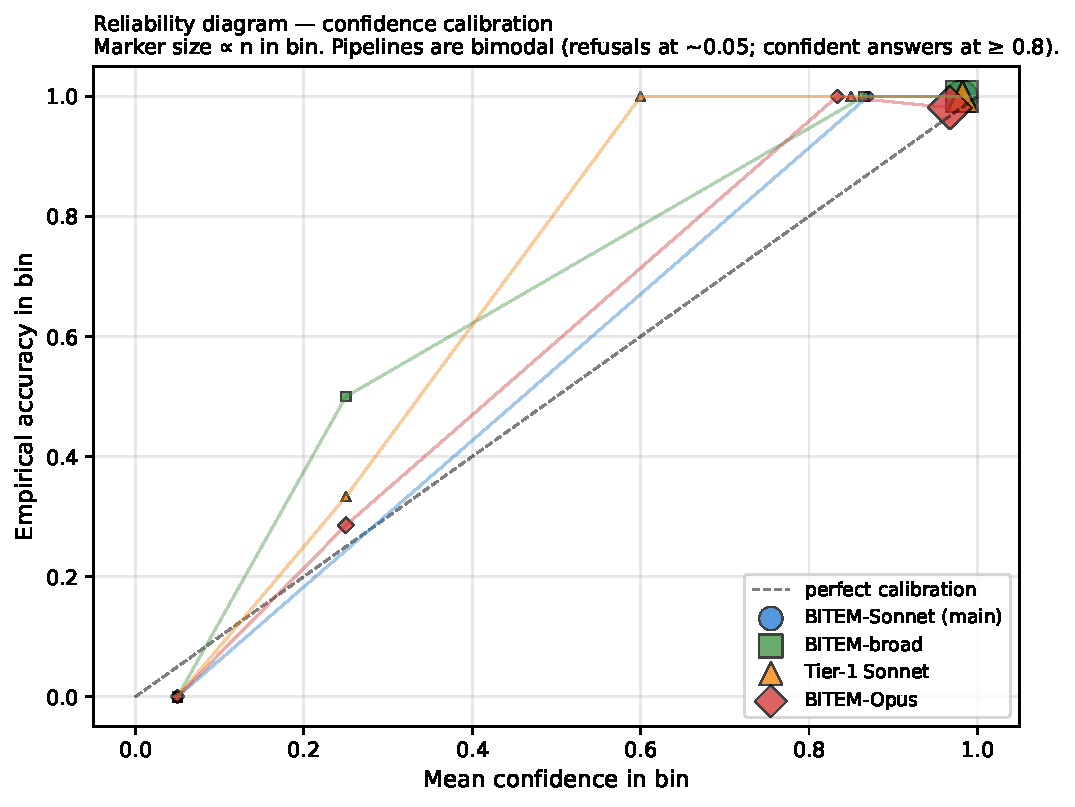
\includegraphics[width=0.82\columnwidth]{figures/fig_reliability.pdf}
\caption{Reliability diagram for retrank's submitted runs (main system AC-2 highlighted):
reported confidence vs.\ empirical accuracy per bin. Confidence tracks accuracy
(near-diagonal), not merely in the mean.}
\label{fig:reliability}
\end{figure}

We stress that we did \emph{not} win by being modest~\cite{modesty}. Our winning runs answer $\sim\!95\%$
of topics correctly at high confidence; the always-refuse strategy that also scores high
\HMR{} does so at near-zero accuracy, whereas we reach top \HMR{} \emph{with} the field's
best accuracy. The $2\times$ \HMR{} gap over BITEM at comparable accuracy (Table~1)
supports calibration as the main differentiator among high-accuracy systems.

\paragraph{The $\RO$ bottleneck.} Why does calibration dominate? Across our 16 development
configurations $\RU$ occupies a narrow high band ($[0.79,0.98]$) while $\RO$ ranges widely
($[0.45,0.95]$), so at this operating point \HMR{} is far more sensitive to $\RO$. The
official scores confirm it: across our four submitted runs $\RU\in[0.96,1.00]$ but
$\RO\in[0.79,0.95]$, and \HMR{} tracks $\RO$. Every winning design choice we identify ---
verifier-anchored confidence, answer-conditional refinement, refusal on weak evidence ---
primarily \emph{raises $\RO$} (suppresses high confidence on wrong answers) rather than
lifting $\RU$. The practical lesson for confidence-scored RAG is therefore asymmetric:
\emph{engineer to suppress confident errors, not to make correct answers more confident.}

\paragraph{What overconfidence looks like.} BITEM's best-\HMR{} run (BITEM-AC-2, the run in
our core comparison) makes the failure concrete. Its confidence
distribution is neither flat nor trivial --- confidences span $0$--$100$ with mean $83.5$
--- but it is systematically \emph{high}: the median is $97$ and $46\%$ of answers carry
confidence $100$. Near-maximal confidence on the $\sim\!8\%$ of topics it answers wrong is
enough to collapse $\RO$ to $0.35$, halving \HMR{} despite $0.92$ accuracy. The calibration
failure is genuine, systematic overconfidence, not an artefact of a degenerate
strategy --- which is exactly what the thesis predicts.

\begin{table}[t]
\caption{The two failure modes. $\RO$ collapses under overconfidence (low accuracy at high
confidence); $\RU$ collapses under sandbagging (near-zero confidence). retrank keeps both
high. (Representative official runs.)}
\label{tab:failure}
\small
\begin{tabular}{llcccc}
\toprule
Run & mode & conf. & acc. & $\RO$ & $\RU$ \\
\midrule
retrank-AC-1  & calibrated     & 0.956 & 0.953 & 0.95 & 1.00 \\
ORG-AC-1      & overconfident  & 0.905 & 0.531 & 0.09 & 0.90 \\
hit-u-AC-4    & sandbagging    & 0.016 & 0.813 & 0.99 & 0.02 \\
\bottomrule
\end{tabular}
\end{table}

\subsection{The win is the pipeline, not the pool}
\label{sec:pool}
Our winning runs use \emph{BITEM's} passages, not our own. Our own PR runs ranked
\emph{last of 22} on nDCG@20 under the AC-derived relevance labels ($0.09$--$0.11$ vs.\
$0.44$ for the top run). More strikingly, phase-1 and phase-2 standing are strongly
\emph{anti}-correlated across the six teams with both a PR and an AC run (Spearman
$\rho_s\approx-0.94$; slr2c2 is omitted for lack of a comparable PR run): the best retriever
(hit-u, PR rank 1) is the worst answerer (AC rank last), and the worst retriever (retrank)
wins AC. We read this with care: because PR is re-scored by how
often AC systems cited each passage, and our AC preferentially cited BITEM's passages, the
inversion is partly a \emph{mechanical} consequence of citation choices rather than an
independent measure of retrieval quality --- we therefore do not claim retrieval was
useless. The defensible, weaker conclusion is that \emph{phase-1 standing did not transfer
to phase-2}: our advantage rode on the pipeline operating over a competitor's pool, not on
our own retrieval. Consistently, adding weaker passages to the strong
BITEM pool (a ten-run multi-team pool) \emph{lowered} \HMR{} from $0.963$ to $0.868$:
dilution, not enrichment.

\begin{table}[t]
\centering\small
\caption{Phase-1 (PR) and phase-2 (AC) standing are strongly anti-correlated across the six
teams with both runs (Spearman $\rho_s\approx-0.94$): the best retriever answers worst, and
retrank (last on PR) wins AC.}
\label{tab:prac}
\begin{tabular}{lcc}
\toprule
Team & best PR nDCG@20 (rank) & best AC \HMR{} (rank) \\
\midrule
hit-u & 0.438 (1) & 0.184 (last) \\
BITEM & 0.422 (2) & 0.492 \\
Error404 & 0.346 (3) & 0.518 \\
WaterlooClarke & 0.318 (4) & 0.761 \\
ORG & 0.309 (5) & 0.760 \\
\textbf{retrank} & \textbf{0.114 (last)} & \textbf{0.974 (1)} \\
\bottomrule
\end{tabular}
\end{table}

\subsection{Internal ablations}
\label{sec:ablations}
Beyond the cross-team comparison, a development sweep over 16 base configurations
(val250-tuned) isolates which design choices move \HMR{}, and confirms they act through
$\RO$. We grade each by whether its $95\%$ bootstrap CI on $\Delta\HMR{}$ excludes zero
(percentile intervals from $B{=}5000$ topic-level resamples, recomputing $\RO$, $\RU$, and
\HMR{} within each resample, with contrasts paired on topics). Because these contrasts are
drawn from an exploratory sweep, the intervals are descriptive and \emph{not}
multiplicity-adjusted; we label the evidence grade accordingly.
\begin{description}
  \item[Robust.] Per-stage model tier matters most at the candidate-answer stage
    ($\Delta\HMR{=}{-}0.13$ Sonnet$\to$Haiku, CI excludes zero) and least at the verifier
    ($-0.05$); the all-Sonnet$\to$all-Haiku regression ($-0.17$) and the naive-pooling
    regression are also robust.
  \item[Suggestive.] Answer-conditional pool refinement helps ($+0.085$, CI
    $[-0.045,+0.44]$); a strong single-team pool beats naive multi-team pooling
    ($-0.11$, CI $[-0.46,+0.04]$) --- an effect of pool \emph{quality}, not count.
  \item[Preliminary.] Answer-first beats nugget-first on a 20-topic head-to-head (equal
    accuracy, $-0.29$ \HMR{} for nugget-first, \emph{entirely} attributable to $\RO$).
\end{description}
\noindent \emph{Verifier-based abstention} is context-dependent: on a noisy multi-team pool
it adds $+0.04$ \HMR{} over never abstaining, but on the clean BITEM pool it adds nothing.
The win on our submitted (clean-pool) runs therefore comes from confidence \emph{calibration},
not abstention per se --- and every one of these levers moves $\RO$, corroborating the
bottleneck of \S\ref{sec:calib}.

\section{Robustness to LLM-Based Evaluation}
\label{sec:judge}
Every R2C2 team used large language models: the task is LLM-based RAG and the rules place
no restriction on model choice, so using an LLM --- Claude included --- is not an advantage
anyone can contest. The legitimate questions are therefore not about \emph{permission} but
about \emph{validity} and \emph{attribution}: (i) whether an evaluation whose ground truth
is itself LLM-generated (Qwen-3.5, GPT-5.5) yields trustworthy scores, and (ii) whether our
margin reflects our method or merely raw model strength. We address both.

\paragraph{Objection A: shared-judge bias.} \emph{``You optimised to an LLM, and the judges
are LLMs.''} We tuned against a Claude self-evaluator; the official labels come from
\emph{Qwen-3.5 and GPT-5.5}. These are different model families, so any agreement is not
self-agreement. Our Claude self-evaluator predicted the \emph{official} \HMR{} of our two
main runs to within $\mathbf{0.0004}$ (self $0.974/0.963$ vs.\ official $0.9744/0.9626$).
Cross-family agreement at this precision is evidence that the calibration we optimised is
real signal, not an artefact of a judge scoring its own family. We report the same
self-vs-official comparison for our other runs, where agreement is looser
($\le 0.02$), and we are explicit (\S\ref{sec:limits}) that the two tightest points are
runs we tuned against, so this is corroborating rather than held-out evidence.

\paragraph{A held-out test: predicting competitors' \HMR.} To break the circularity, we
scored five competitor runs we did \emph{not} tune against --- spanning the official \HMR{}
range --- with a lightweight version of our Claude self-evaluator and compared its
predictions to the official Qwen/GPT scores (Table~\ref{tab:heldout}). Agreement is
\emph{weak}: Spearman $\rho{=}0.60$ but on only $n{=}5$ runs, so it is not significant
(exact permutation $p{\approx}0.35$); mean absolute error is $0.12$, with three of five runs
predicted within $0.01$--$0.13$ and one large miss (slr2c2, whose well-calibrated
low-confidence strategy our simplified judge under-scored). The self-evaluator therefore
shows a non-circular but statistically weak cross-family \emph{signal} --- it orders the
extremes correctly --- rather than demonstrated validity, and it is \emph{not} tightly
calibrated on other teams' runs. We treat it as a small diagnostic: the near-perfect
agreement on our own runs above partly reflects tuning, whereas the held-out agreement is
positive in this sample but not statistically established.

\begin{table}[t]
\centering\small
\caption{Held-out cross-family check: our (lightweight) self-evaluator's predicted \HMR{}
vs.\ the official Qwen/GPT \HMR{} on five competitor runs we did not tune against
(weak, $n{=}5$: $\rho{=}0.60$, permutation $p{\approx}0.35$, MAE $0.12$).}
\label{tab:heldout}
\begin{tabular}{lcc}
\toprule
Competitor run & our self-eval & official \\
\midrule
WaterlooClarke-AC-2 & 0.750 & 0.761 \\
hit-u-AC-1          & 0.187 & 0.184 \\
Error404-AC-3       & 0.504 & 0.518 \\
BITEM-AC-2          & 0.621 & 0.492 \\
slr2c2-AC-4         & 0.286 & 0.729 \\
\bottomrule
\end{tabular}
\end{table}

\paragraph{Within-family judge stability.} We additionally re-judged all four submitted runs
with a second Claude judge (Opus 4.7). Run ordering is preserved and the two main runs move
by $\le0.001$ \HMR; only the hedged runs move materially (AC-3 $+0.03$, AC-4 $+0.06$
Sonnet$\to$Opus), and the official scores fall between the two judges' estimates --- judge
disagreement is concentrated on the hedged runs, not the main system.

\paragraph{Objection B: you just used a stronger model.} If raw model capability drove the
win, scaling the model up should help. It does not: with prompts held fixed (developed on
Sonnet), an \emph{all-Opus} pipeline \emph{regressed} \HMR{} by $0.18$ and an
\emph{all-Haiku} pipeline by $0.17$ (self-eval; bootstrap CIs exclude zero). We read these
cautiously --- because prompts are not re-tuned per tier, they measure \emph{naive model
substitution}, not intrinsic capability (\S\ref{sec:limits}), so we do \emph{not} claim a
larger model is worse. Decomposing the Opus regression makes the mechanism precise: it is
concentrated in the overconfidence reward ($\Delta\RO{=}{-}0.27$), \emph{not} accuracy
($\Delta\text{Acc}{=}{-}0.05$). Opus answers nearly as accurately, but under the
Sonnet-tuned verifier prompt its confidence fails to separate right from wrong answers ---
and this does not recover under post-hoc recalibration (\HMR{} $0.79\!\to\!0.78$), so it is
a confidence-\emph{discrimination} effect localised to the verifier, not inferior
answering. The claim we rely on is one-directional and deliberately weak: subtracting the all-Haiku
penalty from our main system still leaves \HMR{} $\approx0.79$, near the best
non-retrank run ($0.761$) --- \textbf{our actual pipeline, run on the cheapest Claude tier,
would stay in the competitive range of the field-leading team}. The $\sim0.03$ margin is far
smaller than our self-evaluator's cross-family error on held-out competitor runs
(MAE $0.12$, \S\ref{sec:judge}), so we do \emph{not} claim even parity --- only that a far
cheaper model keeps the pipeline near the top of the field, so the margin is not bought by
model strength.

\paragraph{Objection C: you overfit to the test set.} We selected the pipeline's
parameters (notably the abstention threshold) on \textbf{val250}, $248$ held-out synthetic
topics, and never on the 65 official topics (\S\ref{sec:method}). The official set was thus
held out from configuration selection, and the tight self-vs-official agreement above is
measured on topics not used to choose thresholds. This does not escape the LLM loop --- the
synthetic topics are themselves Claude-generated --- but it does rule out fitting to the
specific test topics or their specific official-judge outputs.

\paragraph{Why this is a calibration layer, not a model.} Objection B's ablations show the
gain is not bought by raw model strength; Section~\ref{sec:calib} shows it is in the
confidence layer; and BITEM demonstrates that a comparable answer engine without that layer
scores half our \HMR. The natural reading is that the lever is a \emph{model-agnostic
calibration wrapper}. We test this directly.

We test this two ways: a controlled calibration-transfer experiment (below) and a no-LLM
lower bound (\S\ref{sec:nollm}).

\subsection{Calibration transfer across systems}
\label{sec:transfer}
The no-LLM committee swaps both the answerer and the calibrator's form; a cleaner test of
whether \emph{our specific confidence layer} is the moat is to hold a competitor's answers
fixed and replace only their confidence with ours. For five competitor runs we ran our
verifier (Stage 4) on their submitted answers and applied our Stage-5 rule, then re-scored
\HMR{} under our self-evaluator (Table~\ref{tab:transfer}; the official judge cannot be
re-run). We \emph{quarantine} slr2c2: although it shows the largest gain ($+0.38$), it is
exactly the run our self-evaluator mis-scores worst (Table~\ref{tab:heldout}: self $0.29$
vs.\ official $0.73$), so a gain measured inside that unreliable regime cannot be trusted and
we exclude it from the summary. Across the other four teams our layer improves \HMR{} for
three and the mean gain is $+0.065$, concentrated on the \emph{overconfident} systems
(Error404 $+0.14$, BITEM $+0.13$) with essentially no change for the already-calibrated
WaterlooClarke ($+0.01$). The lone regression is the sandbagger hit-u ($-0.02$): our layer
only \emph{suppresses} overconfidence, so it cannot help a system that is already
under-confident --- exactly the asymmetry the $\RO$ bottleneck predicts. Baselines differ
slightly from Table~\ref{tab:heldout} because the two lightweight evaluators use different
correctness prompts, but the within-experiment original-vs-transfer comparison holds the
evaluator fixed, so it is unaffected by that baseline offset --- though, like every delta
here, it remains \emph{conditional on the surrogate's correctness labels}: a fixed judge
guarantees ON and OFF share labels, but shared Claude-family agreement between our verifier
and self-evaluator could still flatter the layer. Because the answers come from other teams'
systems, this is controlled evidence that the confidence wrapper transfers across systems
\emph{under our self-evaluator}; genuine cross-base-model-family transfer within our own
pipeline remains unproven.

\begin{table}[t]
\centering\small
\caption{Calibration transfer: holding each competitor's \emph{answers} fixed and replacing
only their confidence with our verifier-capped layer. Our layer raises \HMR{} for the
overconfident teams (via $\RO$) and cannot help the sandbagger (hit-u). slr2c2 is quarantined
(our self-evaluator mis-scores it; see text). Scored under our self-evaluator, not the
official judge; $\Delta$\HMR{} is computed from unrounded values.}
\label{tab:transfer}
\begin{tabular}{lcccc}
\toprule
Team run & Acc & \HMR{} orig & \HMR{} $+$layer & $\Delta$\HMR \\
\midrule
slr2c2-AC-4         & 0.68 & 0.243 & 0.619 & \textbf{$+$0.376} \\
Error404-AC-3       & 0.71 & 0.553 & 0.697 & $+$0.144 \\
BITEM-AC-2          & 0.92 & 0.599 & 0.725 & $+$0.125 \\
WaterlooClarke-AC-2 & 0.83 & 0.820 & 0.827 & $+$0.007 \\
hit-u-AC-1 (sandbag)& 0.81 & 0.197 & 0.179 & $-$0.018 \\
\bottomrule
\end{tabular}
\end{table}

\subsection{Base-model swap: the pipeline on GPT}
\label{sec:gptswap}
The transfer test above keeps each competitor's answers fixed and swaps only the confidence
layer; the stronger test is to run the pipeline \emph{end-to-end} with a \emph{non-Claude}
answer/verifier model. We reimplemented a \emph{streamlined} version (candidate $\to$ nuggets $\to$ verifier
$\to$ Stage-5, using the top-20 pool passages by rank \emph{without} the submitted system's
cross-encoder re-rank, 50-passage cap, or Stage-3 entailment filter) with three OpenAI models
on the 65 topics and BITEM pool, scoring correctness with a fixed GPT-5.5 judge
(Table~\ref{tab:gptswap}). The ON and OFF runs share identical answers, nuggets, and
correctness labels (including refusals) and differ \emph{only} in confidence; holding the
judge fixed keeps those labels constant across ON/OFF, so the paired \HMR{} delta isolates the
calibration rule. All three models improve, always via $\RO$ --- the same signature as Claude.
The direction is consistent (3/3 positive) but the per-model effects are \emph{underpowered}:
because the two GPT-5.6 variants are $\ge93\%$ accurate they have only $3$--$4$ incorrect
answers to recalibrate, so their $\RO$ gains are positive with $95\%$ bootstrap CIs that cross
zero; only GPT-4.1-mini (more errors, larger effect) is individually significant. Further
caveats: correctness is scored by a GPT judge, not the official Qwen$+$GPT ensemble, so
absolute \HMR{} here is context, not a like-for-like ranking (only GPT-4.1-mini-ON reaches the
field's $0.761$; none reaches our Claude $0.963$). The claim we draw is narrow and supported:
the verifier-cap rule improves \HMR{} across three GPT configurations under a fixed surrogate
judge --- cross-family evidence (from Claude) that the calibration mechanism is not a Claude
artefact. As with the Claude self-evaluator, a GPT judge scoring GPT answerers may share
family-level agreement, so this is cross-family from Claude but not judge-independent.

\begin{table}[t]
\centering\small
\caption{Base-model swap: streamlined pipeline run on three OpenAI models (fixed GPT-5.5
judge). Calibration raises \HMR{} for all three, always via $\RO$; $\Delta\HMR{}$ with $95\%$
paired-bootstrap CI ($^\ast$ excludes zero). Direction consistent (3/3) but only GPT-4.1-mini
is individually significant --- the accurate GPT-5.6 variants have too few errors to power the
test. $\Delta\HMR{}$ is computed from unrounded values. Model ids as exposed on the account.}
\label{tab:gptswap}
\begin{tabular}{lcccc}
\toprule
Answer/verifier model & Acc & \HMR{} off & \HMR{} on & $\Delta$\HMR{} [95\% CI] \\
\midrule
gpt-5.6-sol    & 0.939 & 0.444 & 0.599 & $+$0.156 [$-$0.03,$+$0.63] \\
gpt-5.6-luna   & 0.954 & 0.577 & 0.717 & $+$0.140 [$-$0.04,$+$0.49] \\
gpt-4.1-mini   & 0.923 & 0.399 & 0.899 & $+$0.500 [$+$0.10,$+$0.81]$^\ast$ \\
\midrule
mean           & --- & --- & --- & $+$0.265 \\
\bottomrule
\end{tabular}
\end{table}

\subsection{A No-LLM Lower Bound}
\label{sec:nollm}
We rebuilt the pipeline with \textbf{no generative model}: a cross-encoder
reranker~\cite{monobert} over the winning pool, a \emph{committee} of extractive QA
encoders (RoBERTa~\cite{roberta}, ELECTRA~\cite{electra}, MiniLM~\cite{minilm},
BERT, TinyRoBERTa, all SQuAD2~\cite{squad2}) that vote span-by-span, and a
confidence calibrator over the answerability margin and committee agreement, fit on
the held-out synthetic val250 set. This calibrate-then-abstain design follows Kamath
et al.~\cite{kamath2020}, who train a classifier to predict QA errors; we extend it
to the AC/\HMR{} setting.

\paragraph{Voting scales accuracy, then plateaus.} Committee voting --- a discrete
analogue of self-consistency~\cite{selfconsistency} --- raises accuracy from $0.42$
(one model) to $0.52$ (three), then saturates: a fourth and fifth answerer add
nothing (Table~\ref{tab:nollm}), so the extractive ceiling is $\approx0.52$.
Per-answer calibration degrades as the committee grows (margin AUC $0.85$ at two
answerers to $0.74$ at five; Table~\ref{tab:nollm}), so \HMR{} peaks at a two-model
committee. At answer-everything the committee scores \HMR{} $0.66$ \emph{under our
self-evaluator}. Because this is a surrogate score, not an official run, we do not insert it
into the official ranking; but scored by the \emph{same} self-evaluator, the committee
(\HMR{} $0.66$, Acc $0.52$) draws level with the far more accurate BITEM (\HMR{} $0.62$
under the same judge, Table~\ref{tab:heldout}; Acc $0.92$, Table~\ref{tab:transfer}). This is the calibration thesis in
miniature: a \emph{calibrated but inaccurate} system matches
an \emph{accurate but overconfident} one, under a fixed judge, precisely because \HMR{}
rewards the alignment of confidence with correctness, not correctness itself.

\paragraph{Which non-LLM techniques help?} Table~\ref{tab:sweep} sweeps the
techniques available without a generative model. \emph{Confidence is aleatoric and
cheap}: the answerability margin predicts correctness at AUC up to $0.85$ (two-model
committee), and adding second-order feature interactions --- in the spirit of
SmoothHess~\cite{smoothhess} and integrated-Hessian~\cite{inthessians} interaction analysis
--- lifts the larger (three-model) committee's margin AUC from $0.766$ to $0.803$
(Table~\ref{tab:sweep}), but only under strict feature parsimony. \emph{Every variance-based
uncertainty estimator failed}: MC-dropout~\cite{gal2016} (AUC $0.53$), deep-ensemble
score dispersion~\cite{ensembles2017} (AUC $0.51$); a last-layer Laplace
approximation~\cite{laplace2021} targets the identical posterior-predictive variance and so
we predict it behaves the same, though we did not run it.
The useful signal is the point estimate, not its spread. \emph{Abstention should be
coverage-controlled} (conformal~\cite{conformal2023,mohri2024}), not \HMR-maximised
--- the latter games the metric to answering $17\%$ of topics at $0.14$ accuracy.
\emph{Accuracy needs scale}: a small generative reader (flan-t5-base~\cite{flant5})
reaches only $0.48$, \emph{below} the extractive committee, over-generalising where
extraction stays precise.

\textbf{So the LLM's measured contribution is answer accuracy at scale} --- not the
confidence layer, and not, in these experiments, alignment with an LLM judge. ``You only won because you
used a strong LLM'' reduces to ``the LLM answers harder questions,'' which is the
task.

\paragraph{Statistical power.} Following Sakai's advocacy for reporting significance
and power rather than bare point estimates~\cite{sakai-reform,sakai-sigtest}, we
apply the randomised Tukey HSD test~\cite{sakai-sigtest} ($B{=}5000$) to the committee
ladder. The voting gain from one to three answerers is \emph{suggestive but not
significant} ($\Delta\text{Acc}{=}{+}0.108$, $p{=}0.14$): voting fixes 12 wrong
single-model answers but breaks 5 correct ones (net ${+}7/65$). A simulation-based
power analysis shows the minimum accuracy difference detectable at $n{=}65$ with
$80\%$ power is $\approx0.15$ --- above the observed gain --- so this collection lacks the
power to detect an effect of the observed size; the result is inconclusive, not a
demonstrated null. We therefore report it as a trend; only the $0.52\!\to\!0.94$
committee-vs-LLM accuracy gap (both self-evaluated on $n{=}65$) far exceeds the detectable
threshold, so it is robust to the judge and to the $64$-vs-$65$-topic denominator.

\paragraph{Per-topic failure analysis.} Following the organisers' request for
per-topic analysis, we heuristically type the 65 questions (rule-based, no LLM) and
compare committee and LLM accuracy by type (Table~\ref{tab:pertype}). The LLM
dominates \emph{every} type, but its advantage is largest exactly where reasoning is
required: on \emph{count} questions (``how many\ldots''), which need an aggregation
no extracted span can express, the committee collapses to $0.29$ against the LLM's
$0.86$. Even on plain factoids the committee reaches only $0.59$ (LLM $1.00$),
because the answer is not always a clean extractable span. No question type is
competitive for extraction; the generative advantage is pervasive and peaks on
aggregation --- a concrete localisation of the reasoning gap.

\begin{table}[t]
\centering\small
\caption{Per-type accuracy (both systems self-evaluated on the 65 typed topics),
committee-3 vs.\ LLM (rule-based typing). The LLM leads on every type; its margin is largest
on count/aggregation questions.}
\label{tab:pertype}
\begin{tabular}{lccc}
\toprule
Question type & $n$ & committee & LLM \\
\midrule
factoid & 27 & 0.59 & 1.00 \\
person  & 19 & 0.58 & 0.95 \\
count (``how many'') & 14 & \textbf{0.29} & 0.86 \\
title   & 5  & 0.60 & 0.80 \\
\bottomrule
\end{tabular}
\end{table}

\begin{table}[t]
\centering\small
\caption{No-LLM committee ladder (answer-everything). Voting scales accuracy to a
$\approx0.52$ plateau; \HMR{} peaks at a two-model committee as calibration degrades.
Committee rows are self-evaluated ($n{=}65$); the LLM pipeline row is official ($n{=}64$;
our self-eval agrees with official to $0.0004$, \S\ref{sec:judge}), shown for reference.}
\label{tab:nollm}
\begin{tabular}{lccc}
\toprule
System & Accuracy & \HMR & margin AUC \\
\midrule
Committee-1 (RoBERTa) & 0.415 & 0.629 & 0.849 \\
Committee-2 (+ELECTRA) & 0.462 & \textbf{0.677} & 0.85 \\
Committee-3 (+MiniLM) & \textbf{0.523} & 0.659 & 0.766 \\
Committee-5 (+BERT,+TinyRoBERTa) & 0.523 & 0.644 & 0.736 \\
\midrule
LLM pipeline (retrank-AC-2) & 0.953 & 0.963 & --- \\
\bottomrule
\end{tabular}
\end{table}

\begin{table}[t]
\centering\small
\caption{Non-LLM technique sweep (self-evaluated surrogate, $n{=}65$). Confidence is
recovered cheaply; variance-based uncertainty fails; accuracy needs scale.}
\label{tab:sweep}
\begin{tabular}{llc}
\toprule
Technique & Metric & Result \\
\midrule
Committee voting (1$\to$3) & Accuracy & 0.42$\to$0.52 (plateau) \\
Interaction calibrator (2nd-order) & disc.\ AUC & 0.766$\to$\textbf{0.803} \\
Discrete agreement & AUC & 0.76 \\
Ensemble score-variance & AUC & 0.51 \\
MC-dropout variance & AUC & 0.53 \\
Last-layer Laplace & \emph{untested} & pred.\ $\approx$0.5 \\
Conformal abstention & --- & coverage knob \\
Small generative reader (flan-t5) & Accuracy & 0.48 ($<$0.52) \\
\bottomrule
\end{tabular}
\end{table}

\section{What Did Not Work}
\label{sec:negative}
Four interventions we expected to help, hurt. \emph{(The model-tier ablations below are
self-evaluated and hold prompts fixed at their Sonnet-developed form, so they measure naive
substitution under our judge, not intrinsic model capability --- see \S\ref{sec:limits}.)}
(1) \emph{Scaling up.} An all-Opus pipeline regressed \HMR{} by $0.176$. Decomposition is
instructive: the drop is almost entirely in the overconfidence reward ($\Delta\RO{=}{-}0.27$),
not accuracy ($\Delta\text{Acc}{=}{-}0.05$) --- Opus answers nearly as well but, under the
Sonnet-tuned verifier prompt, reports high confidence on its errors, and this does not
recover under post-hoc recalibration ($0.79\!\to\!0.78$). The regression is confidence
\emph{discrimination} at the verifier, not answer quality.
(2) \emph{Scaling down.} All-Haiku regressed by $0.170$; the useful configuration is
\emph{selective} tiering --- a strong model at the candidate-answer stage (the most
model-sensitive, $\Delta\HMR=-0.13$ Sonnet$\to$Haiku) and cheaper models downstream (the
verifier is least sensitive, $-0.05$) --- not uniform scale in either direction.
(3) \emph{Naive multi-team pooling.} Enlarging the strong single-team pool with weaker
passages lowered \HMR{} ($0.963\!\to\!0.868$); more evidence was dilution, not enrichment.
(4) \emph{Per-topic oracle pool selection.} Picking, per topic, the pool whose verifier
most strongly agreed with its candidate --- an apparently free ``oracle'' --- also reduced
\HMR: verifier agreement is a good \emph{ranking} signal but a biased \emph{selection}
criterion, favouring confidently-wrong candidates on hard topics.

\section{Limitations}
\label{sec:limits}
We are deliberately conservative about what the result does and does not show.
\begin{itemize}
  \item \textbf{LLM-judged ground truth.} Accuracy, \MNP, and \HMR{} all rest on
    model-generated labels (Qwen-3.5, GPT-5.5). Our cross-family agreement (\S\ref{sec:judge})
    mitigates but does not eliminate the concern; none of these numbers are human-validated.
  \item \textbf{Self-evaluator validation is partly in-sample.} The tightest self-vs-official
    agreement is on runs we tuned against the self-evaluator. A fully non-circular test is
    to predict \emph{other teams'} official \HMR{} from our self-evaluator; we report this
    where data permit and flag it as the cleaner validation.
  \item \textbf{Synthetic tuning data is also LLM-generated.} val250 mitigates overfitting
    to the 65 official topics, but the synthetic topics were produced by Claude (Sonnet
    generator, Haiku in-loop judge), so tuning generalisation is demonstrated within a
    Claude-imagined distribution, not against human-authored topics.
  \item \textbf{Cross-family transfer is now shown, under a surrogate judge.} The calibration
    layer's model-agnosticism is demonstrated two ways: the calibration-transfer experiment
    (\S\ref{sec:transfer}) lifts three of four non-quarantined \emph{other teams'} runs, and the base-model
    swap (\S\ref{sec:gptswap}) reproduces the calibration gain when the \emph{streamlined}
    pipeline runs end-to-end on three GPT models (3/3 positive $\Delta\HMR$). The residual caveat is the judge:
    both are scored by our own self-evaluator or a GPT judge, not the official Qwen$+$GPT
    ensemble, which we cannot re-run. A non-Claude pipeline scored by the official judge is
    the only piece still outside our reach.
  \item \textbf{Model-tier ablations hold prompts fixed.} The all-Opus and all-Haiku
    configurations reuse the prompts developed on Sonnet, changing only the model. The
    resulting regressions therefore measure \emph{naive model substitution without
    re-tuning}, not intrinsic model capability; we do not claim Opus is intrinsically
    worse, only that the pipeline is co-adapted to its model and cannot be re-tiered for
    free. The complementary claim --- that our (Sonnet-prompted) pipeline run \emph{on
    Haiku} would remain \emph{competitive with the field-leading team} (in the field's competitive range, not a decisive lead) --- is unaffected, since it evaluates the actual
    deployed pipeline on a cheaper model.
  \item \textbf{Small sample and evidence grades.} $n=64$ topics. Some findings are
    suggestive (answer-conditional refinement, CIs cross zero) or preliminary
    (answer-first vs.\ nugget-first, 20 topics); we mark them as such rather than
    headlining them.
\end{itemize}

\section{Reproducibility}
\label{sec:repro}
We release code and data; the operational specifics are:
\textbf{Pool.} BITEM-PG-1 $+$ BITEM-PG-2, deduplicated by \texttt{(doc\_id, 64-char prefix)},
re-ranked by \texttt{cross-encoder/ms-marco-MiniLM-L-12-v2}, capped at 50 passages.
\textbf{Models.} Claude Sonnet 4.6 at all stages of the submitted runs; Haiku 4.5 / Opus 4.7
for the tier ablations; the self-evaluator is Sonnet 4.6 with Opus 4.7 cross-validation.
\textbf{Verifier (Stage 4).} A separate call re-derives an answer from the \emph{entailed
nuggets only} and compares it to the candidate, emitting \texttt{match\_score}$\in\{0,1,2\}$
($0$ disagree/refuse, $1$ partial, $2$ full).
\textbf{Confidence (Stage 5), the exact rule.} If there are no entailed nuggets or the answer
is empty, refuse (\texttt{conf}$=5$); else cap the model's self-confidence at $25$ if
\texttt{match\_score}$=0$, at $60$ if $=1$, and leave it unchanged if $=2$. The abstention
behaviour and configuration were selected on val250; the 65 official topics were never used
for tuning.

\section{Related Work}
\label{sec:related}
\textbf{Confidence-scored answering and modesty.} \HMR{} and the ``modesty'' framing of
over- and under-confidence are due to Sakai and the R2C2 organisers~\cite{sakai-hmr,modesty,brevrag};
unlike aggregate calibration measures such as expected calibration error~\cite{guo2017},
\HMR{} penalises the two error directions separately. Our paper is a case study in optimising
it.
\textbf{Selective prediction and abstention.} Deciding \emph{when} to answer has a long
history~\cite{kamath2020}: Kamath et al.\ train a classifier over model features to predict
errors and abstain --- the design our no-LLM calibrator follows. Conformal
prediction~\cite{conformal2023,mohri2024} gives distribution-free coverage control, which we
explore as a principled alternative for setting abstention thresholds; the submitted runs
used \HMR-maximised thresholds selected on val250.
\textbf{Calibration and uncertainty.} Post-hoc calibration~\cite{guo2017} and Bayesian
uncertainty --- MC-dropout~\cite{gal2016}, deep ensembles~\cite{ensembles2017}, and Laplace
approximations~\cite{laplace2021} --- are standard tools; we find that variance-based
estimators we tried (MC-dropout, deep ensembles) add nothing on this task and the
point-estimate margin dominates. Second-order
feature-interaction analysis~\cite{smoothhess,inthessians} inspired our interaction-aware
calibrator. Our retrieval and answering components build on cross-encoder
re-ranking~\cite{monobert} and extractive QA~\cite{squad2,roberta,electra,minilm}.
\textbf{RAG evaluation and LLM judges.} R2C2 pools passages across teams for retrieval-augmented
answering~\cite{rag}. Because its relevance labels and answer judgments are produced by
LLMs~\cite{llmjudge}, we treat judge validity as a first-class concern, and our committee
voting is a discrete analogue of self-consistency~\cite{selfconsistency}.

\section{Conclusion}
R2C2's Answering-with-Confidence subtask is a calibration problem wearing a QA costume. The
teams whose confidence did not track their accuracy
fell into one of two failure modes and lost, sometimes despite excellent retrieval or
competitive accuracy. retrank treated it as calibration from the start: an answer-first
pipeline whose confidence comes from an independent verifier, winning first place on all
three official metrics, with all four of its runs above every non-retrank run on \HMR.
Because the win was scored by LLMs, we tested it against that fact rather than around it, and
found the margin is not explained solely by using the largest Claude tier. Under our
surrogate judges, the calibration layer itself transfers: it lifts three of four
non-quarantined competitors' runs (self-evaluator) and, run on three GPT models (fixed GPT
judge), reproduces the calibration gain (3/3 positive, one significant). What remains --- confirmation under the
\emph{official} Qwen$+$GPT judge, and the residual limitations of \S\ref{sec:limits} (64
scored topics, LLM-generated labels, Claude-tuned thresholds) --- separates a strong
participant result from a fully general method claim.

\begin{thebibliography}{99}
\bibitem{overview} S.~Tao, T.~Sakai, et al. Overview of the NTCIR-19 R2C2 Task. In {\em Proc.\ NTCIR-19}, 2026.
\bibitem{sakai-hmr} T.~Sakai. Evaluating System Responses Based on Overconfidence and Underconfidence. In {\em Proc.\ EVIA / NTCIR-19}, 2025.
\bibitem{sakai-sigtest} T.~Sakai. {\em Laboratory Experiments in Information Retrieval: Sample Sizes, Effect Sizes, and Statistical Power}. Springer, 2018.
\bibitem{sakai-reform} T.~Sakai. Statistical Reform in Information Retrieval? {\em SIGIR Forum}, 48(1):3--12, 2014.
\bibitem{brevrag} T.~Sakai and S.~Tao. BREV-RAG: Beyond Relevance-based EValuation of RAG Systems. In {\em SIGIR-AP (Workshop)}, 2025.
\bibitem{modesty} S.~Tao and T.~Sakai. Evaluating the Modesty of RAG Systems at the NTCIR-19 R2C2 Task: Potential Challenges. In {\em SIGIR-AP BREV-RAG Workshop}, 2025.
\bibitem{kamath2020} A.~Kamath, R.~Jia, and P.~Liang. Selective Question Answering under Domain Shift. In {\em ACL}, 2020.
\bibitem{guo2017} C.~Guo, G.~Pleiss, Y.~Sun, and K.~Q. Weinberger. On Calibration of Modern Neural Networks. In {\em ICML}, 2017.
\bibitem{gal2016} Y.~Gal and Z.~Ghahramani. Dropout as a Bayesian Approximation. In {\em ICML}, 2016.
\bibitem{ensembles2017} B.~Lakshminarayanan, A.~Pritzel, and C.~Blundell. Simple and Scalable Predictive Uncertainty Estimation using Deep Ensembles. In {\em NeurIPS}, 2017.
\bibitem{laplace2021} E.~Daxberger et al. Laplace Redux --- Effortless Bayesian Deep Learning. In {\em NeurIPS}, 2021.
\bibitem{smoothhess} M.~Torop, A.~Masoomi, D.~Erdogmus, and J.~Dy. SmoothHess: ReLU Network Feature Interactions via Stein's Lemma. In {\em NeurIPS}, 2023.
\bibitem{inthessians} J.~D. Janizek, P.~Sturmfels, and S.-I. Lee. Explaining Explanations: Axiomatic Feature Interactions for Deep Networks. {\em JMLR}, 22, 2021.
\bibitem{conformal2023} A.~N. Angelopoulos and S.~Bates. A Gentle Introduction to Conformal Prediction and Distribution-Free Uncertainty Quantification. {\em Foundations and Trends in ML}, 2023.
\bibitem{mohri2024} C.~Mohri and T.~Hashimoto. Language Models with Conformal Factuality Guarantees. In {\em ICML}, 2024.
\bibitem{monobert} R.~Nogueira and K.~Cho. Passage Re-ranking with BERT. {\em arXiv:1901.04085}, 2019.
\bibitem{squad2} P.~Rajpurkar, R.~Jia, and P.~Liang. Know What You Don't Know: Unanswerable Questions for SQuAD. In {\em ACL}, 2018.
\bibitem{roberta} Y.~Liu et al. RoBERTa: A Robustly Optimized BERT Pretraining Approach. {\em arXiv:1907.11692}, 2019.
\bibitem{electra} K.~Clark, M.-T. Luong, Q.~V. Le, and C.~D. Manning. ELECTRA: Pre-training Text Encoders as Discriminators Rather Than Generators. In {\em ICLR}, 2020.
\bibitem{minilm} W.~Wang et al. MiniLM: Deep Self-Attention Distillation for Task-Agnostic Compression. In {\em NeurIPS}, 2020.
\bibitem{rag} P.~Lewis et al. Retrieval-Augmented Generation for Knowledge-Intensive NLP Tasks. In {\em NeurIPS}, 2020.
\bibitem{selfconsistency} X.~Wang et al. Self-Consistency Improves Chain of Thought Reasoning in Language Models. In {\em ICLR}, 2023.
\bibitem{llmjudge} L.~Zheng et al. Judging LLM-as-a-Judge with MT-Bench and Chatbot Arena. In {\em NeurIPS}, 2023.
\bibitem{flant5} H.~W. Chung et al. Scaling Instruction-Finetuned Language Models. {\em arXiv:2210.11416}, 2022.
\end{thebibliography}

\end{document}
